\begin{frame}{Exact Sequences \& Linear Algebra}
Suppose $A \subset X$ then we have:

\[ \begin{tikzcd}[ampersand replacement=\&, column sep=small]
0 \arrow{r} \& C_n(A) \arrow{r}{i} \& C_n(X) \arrow{r}{j} \& C_n(X/A) \arrow{r} \& 0
\end{tikzcd}
\]
This is \emph{exact} meaning that $\ker{j} = \im{i}$. \\
\vspace{.5cm}
When we compute homology we get a larger exact sequence:
\[ \begin{tikzcd}[ampersand replacement=\&, column sep=small]
\ldots \arrow{r}{\delta} \& H_n(A) \arrow{r}{i} \& H_n(X) \arrow{r}{j} \& H_n(X/A) \arrow{r}{\delta} \& H_{n-1}(A) \arrow{r}{i} \& \ldots 
\end{tikzcd}
\]
where:
\[ \delta_n([x]) = [\partial_n(x)] \]

\begin{center}
\textbf{This is the recipe for a basic parallel algorithm.}
\end{center}
\end{frame}
\begin{frame}{Exact Sequences \& Linear Algebra}
We can decompose $\partial_X$ the boundary matrix for $X$ as follows: 
\only<1>{
\[ \begin{blockmatrixtabular}
  \begin{blockmatrixtabular}
  \fblockmatrix     [0.8,1.0,0.8]{1.5in}{1.5in}{$\partial_A$}\\
  \fblockmatrix     [0.8,0.8,1.0]{1.5in}{1.5in}{$0$}
  \end{blockmatrixtabular}
  \begin{blockmatrixtabular}
  \fblockmatrix     [0.8,0.8,1.0]{1.5in}{1.5in}{$\tilde{\delta}$}\\
  \fblockmatrix     [1.0,0.8,0.8]{1.5in}{1.5in}{$\partial_{X/A}$}
  \end{blockmatrixtabular}
\end{blockmatrixtabular} 
\]
}
\only<2>{
\[ \begin{blockmatrixtabular}
  \begin{blockmatrixtabular}
  \fblockmatrix     [0.8,1.0,0.8]{1.5in}{1.5in}{$S_A \cdot P_A$}\\
  \fblockmatrix     [0.8,0.8,1.0]{1.5in}{1.5in}{$0$}
  \end{blockmatrixtabular}
  \begin{blockmatrixtabular}
  \fblockmatrix     [0.8,0.8,1.0]{1.5in}{1.5in}{$\delta = S_{X/A}\tilde{\delta}D_{X/A}$}\\
  \fblockmatrix     [1.0,0.8,0.8]{1.5in}{1.5in}{$P_{X/A}$}
  \end{blockmatrixtabular}
\end{blockmatrixtabular} 
\]
}
The algorithm becomes: 
\begin{enumerate}
\item<1-> Compute homology within each diagonal block (in parallel).
\begin{description}
\item \hspace*{-2cm} Factor $\partial_A = S_A \cdot P_A \cdot D_A$.  where $S$ and $D$ are invertible.
\item \hspace*{-2cm} Factor $\partial_{X/A} = S_{X/A} \cdot P_{X/A} \cdot D_{X/A}$.  
\end{description}
\item<2> Afterwords: reduce the map $\delta$.
\begin{description}
\item \hspace*{-2cm} For each nonzero column in $\delta$ whose reduce them against $S_AP_A$
\end{description}
\end{enumerate}
\end{frame}
\begin{frame}{Algorithm Analysis}
Assume $\card{A} = n$ and $\card{X} = m$

\begin{description}
\item<1->[Correctness] follows from exact sequence.
\item<2->[Complexity] $O((m-n)^3 + n^3 + (m-n) \cdot m \cdot n)$. 
\item<3->[Speedup] This is minimized when $n = \frac{m}{2}$ and at that point we have a speedup of 2.
\end{description}
\only<4>{How to correctly extend this to a sequence of subspaces \[ K_0 \subseteq K_1 \subseteq K_2 \subset \ldots \subset K_n \hspace{.25cm} ?\] }
\end{frame}


\begin{frame}{Homology from a filtration}
How to correctly extend this to a sequence of subspaces \[ K_0 \subseteq K_1 \subseteq K_2 \subset \ldots \subset K_n \hspace{.25cm} ?\] 
We can decompose $\partial_X$ the boundary matrix $X$ in a similar way: 
\[ \begin{blockmatrixtabular}
  \begin{blockmatrixtabular}
    \alt<1>{\greenbox{$\partial_0$}}{\bluebox{$\partial_0$}} \\
    \alt<1>{\bluebox{0}}{\bluebox{0}} \\
    \alt<1>{\bluebox{0}}{\bluebox{0}} \\
    \alt<1>{\bluebox{0}}{\bluebox{0}} \\
    \alt<1>{\bluebox{0}}{\bluebox{0}}
  \end{blockmatrixtabular}
  \begin{blockmatrixtabular}
    \alt<2>{\greenbox{$\tilde{d_0}$}}{\bluebox{$\tilde{d_0}$}} \\
    \alt<1>{\greenbox{$\partial_1$}}{\bluebox{$\partial_1$}} \\
    \alt<1>{\bluebox{0}}{\bluebox{0}} \\
    \alt<1>{\bluebox{0}}{\bluebox{0}} \\
    \alt<1>{\bluebox{0}}{\bluebox{0}}
  \end{blockmatrixtabular}
  \begin{blockmatrixtabular}   
    \alt<3>{\greenbox{$\tilde{d_0}$}}{\bluebox{$\tilde{d_0}$}} \\
    \alt<2>{\greenbox{$\tilde{d_0}$}}{\bluebox{$\tilde{d_0}$}} \\
    \alt<1>{\greenbox{$\partial_2$}}{\bluebox{$\partial_2$}} \\
    \alt<1>{\bluebox{0}}{\bluebox{0}} \\
    \alt<1>{\bluebox{0}}{\bluebox{0}}
  \end{blockmatrixtabular}
    \begin{blockmatrixtabular}
    \alt<4>{\greenbox{$\ldots$}}{\bluebox{$\ldots$}} \\
    \alt<3>{\greenbox{$\ldots$}}{\bluebox{$\ldots$}} \\
    \alt<2>{\greenbox{$\ldots$}}{\bluebox{$\ldots$}} \\
    \alt<1>{\greenbox{$\ldots$}}{\bluebox{$\ldots$}} \\
    \alt<1>{\bluebox{0}}{\bluebox{0}}
    \end{blockmatrixtabular}
    \begin{blockmatrixtabular}
    \alt<5>{\greenbox{$\tilde{d}_{n,n}$}}{\bluebox{$\tilde{d}_{n,n}$}} \\
    \alt<4>{\greenbox{$\tilde{d}_{n-1,n}$}}{\bluebox{$\tilde{d}_{n-1,n}$}} \\
    \alt<3>{\greenbox{$\tilde{d}_{\ldots,n}$}}{\bluebox{$\tilde{d}_{\ldots,n}$}} \\
    \alt<2>{\greenbox{$\tilde{d}_{0,n}$}}{\bluebox{$\tilde{d}_{0,n}$}} \\
    \alt<1>{\greenbox{$\partial_n$}}{\bluebox{$\partial_n$}} \\
  \end{blockmatrixtabular}
\end{blockmatrixtabular} 
\]
\only<6>{\textbf{Question: } How do you show correctness?}
\end{frame}


\begin{frame}{Spectral Sequence of A Filtration}
\only<1-5>{
\begin{figure}
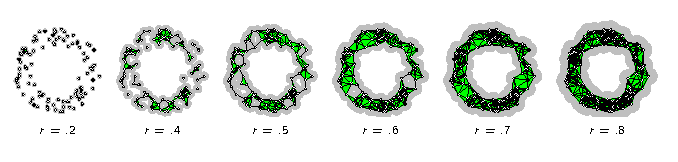
\includegraphics[width=\textwidth]{filtration}
\end{figure}
}
\only<1>{
From our sequence of spaces, we have a filtration of chain complexes:
\[ 
\begin{tikzcd}[ampersand replacement=\&, column sep=small]
0 \arrow{r}{i} \& C_*(K_0) \arrow{r}{i} \& C_*(K_1) \arrow{r}{i}    \& \ldots \arrow{r}{i} \& C_*(K_{n-1}) \arrow{r}{i} \& C_*(K_n) 
\end{tikzcd}
\]
}
\only<2>{
Attach the co-kernel to get short exact sequences
\[
\hspace*{-1cm}
\begin{tikzcd} [ampersand replacement=\&, column sep=small]
0 \arrow{r}{i} \&  C_*(K_0) \arrow{r}{i}\arrow{d}{j} \&  C_*(K_1) \arrow{r}{i}\arrow{d}{j}    \& \ldots \arrow{r}{i} \&  C_*(K_{n-1}) \arrow{r}{i} \arrow{d}{j} \&  C_*(K_n) \arrow{d}{j} \\ 	
\&     C_*(K_0,{0}) \&	C_*(K_1,{K_0}) \& \ldots  	 \& C_*(K_{n-1},{K_{n-2}})		 \& C_*(K_n,{K_{n-1}}) 
\end{tikzcd}
\]
}
\only<3-4>{
Pass to homology, where triangles are exact. \\
\[
\hspace*{-1cm}
\begin{tikzcd}[ampersand replacement=\&, column sep=small]
0 \arrow{r}{i} \& H(K_0 \arrow{r}{i}\arrow{d}{j}) \& H(K_1 \arrow{r}{i}\arrow{d}{j})    \& \ldots \arrow{r}{i} \& H(K_{n-1}) \arrow{r}{i} \arrow{d}{j} \& H(K_n\arrow{d}{j}) \\ 		
\&     H(K_0) \&	  \only<4>{\arrow{l}{d_{1}}} \arrow{ul}{\delta}  H(K_1, {K_0}) \& \only<4>{\arrow{l}{d_{1}}} \arrow{ul}{\delta} \hspace{.5cm} \ldots  	 \&\only<4>{\arrow{l}{d_{1}}}\arrow{ul}{\delta}H(K_{n-1}, {K_{n-2}})		 \& \only<4>{\arrow{l}{d_{1}}} \arrow{ul}{\delta} H(K_n, {K_{n-1}})
\end{tikzcd}
\]
\[  E^2 = H_*(d_1) \]
}
\only<5-6>{
Build a new chain complex by constructing $d_1 = j \circ \delta$ 
\[
\begin{tikzcd}[ampersand replacement=\&, column sep=small]
0 \arrow{r}{i} \& H(K_0 \arrow{r}{i}\arrow{d}{j}) \& H(K_1 \arrow{r}{i}\arrow{d}{j})    \& \ldots \arrow{r}{i} \& H(K_{n-1}) \arrow{r}{i} \arrow{d}{j} \& H(K_n\arrow{d}{j}) \\ 		
\&     E^2_0 \&	  \arrow{l}{0} \arrow{ul}{\delta}  E^2_1 \& \arrow{l}{0} \arrow[bend left]{ll}{d_{2}} \arrow{ul}{\delta} \hspace{.5cm} \ldots  	 \& \arrow{l}{0} \arrow[bend left]{ll}{d_{2}} \arrow{ul}{\delta}E^1_{n-1}	 \& \arrow{l}{0} \arrow[bend left]{ll}{d_{2}} \arrow{ul}{\delta} E_n
\end{tikzcd}
\]
\pause
More generally:
\[ d_{r,p}: E_{r+p} \rightarrow E_p \]
Eventually $d_{n,p} = 0$, when sequence has converged.  
}
\only<7->{
\[
\begin{tikzcd}[ampersand replacement=\&, column sep=small]
0 \arrow{r}{i} \& H(K_0 \arrow{r}{i}\arrow{d}{j}) \& H(K_1 \arrow{r}{i}\arrow{d}{j})    \& \ldots \arrow{r}{i} \& H(K_{n-1}) \arrow{r}{i} \arrow{d}{j} \& H(K_n\arrow{d}{j}) \\ 		
\&     E^\infty_0 \&	  \arrow{l}{0} \arrow{ul}{\delta}  E^\infty_1 \& \arrow{l}{0} \arrow{ul}{\delta} \hspace{.5cm} \ldots  	 \& \arrow{l}{0} \arrow{ul}{\delta}E^\infty_{n-1}	 \& \arrow{l}{0} \arrow{ul}{\delta} E^\infty_n
\end{tikzcd}
\]
The data on the final page is called the $E^\infty$ page.  \\
\pause
\begin{theorem}{Free Lunch}
\[ PH_*(K) \cong  \bigoplus_{r,p} t^p \operatorname{Im}(d_{r,p})/t^{p+r} \bigoplus_p t^p E^\infty_p \]
\end{theorem}
}
\end{frame}
\begin{frame}{Remarks}
\begin{itemize}
\item<1-> Clear connection to persistent homology
\item<2-> Easy to implement
\item<3-> \emph{Doesn't load balance well} (lose a useful thread at each step)
\item<4-> Data on each processor eventually coupled to every other processor.
\end{itemize}
\only<5>{Seek an algorithm which works on large parts of the space in parallel, with small intersections}
\end{frame}